\documentclass[10pt]{article}

% Be sure to use PDF Latex
\pdfoutput=1

% links
\usepackage[bookmarks,bookmarksdepth=2, colorlinks=true, linkcolor=blue,citecolor=red, urlcolor=blue]{hyperref}


\usepackage{fullpage}

\usepackage[latin1]{inputenc}
\usepackage{../mystyle}
\usepackage{wrapfig}


\newcommand{\dims}{d}


\graphicspath{{../figures/}}



\title{Course notes on\\Automatic Differentiation} 

\author{%
\begin{tabular}{c}
	Gabriel Peyr{\'e} \\ CNRS \& DMA \\
	 PSL, \'Ecole Normale Sup\'erieure \\
	 \url{gabriel.peyre@ens.fr}\\
	 \url{https://mathematical-tours.github.io}\\
	 \url{www.numerical-tours.com}
\end{tabular}
}


\date{\today}

\renewcommand{\subsection}[1]{\section{#1}}

%%

\begin{document}

\maketitle

\begin{abstract}
		These are course note on automatic differentiation. They cover the basics of the forward and backward modes, and draw connexions with the adjoint state method. 
\end{abstract}

%
% !TEX root = ../auto-diff/AutoDiff.tex

%%% SECTION PART OF optim-smooth.tex



The main computational bottleneck of gradient descent methods (batch or stochastic) is the computation of gradients $\nabla f(x)$. For simple functionals, such as those encountered in ERM for linear models, and also for MLP with a single hidden layer, it is possible to compute these gradients in closed form, and that the main computational burden is the evaluation of matrix-vector products. For more complicated functionals (such as those involving deep networks), computing the formula for the gradient quickly becomes cumbersome. Even worse: computing these gradients using the usual chain rule formula is sub-optimal. We presents methods to compute recursively in an optimal manner these gradients. The purpose of this approach is to automatize this computational step.  

%%%%%%%%%%%%%%%%%%%%%%%%%%%%%%%%%%%%%%%%%%%%%%%%%%%%%%%%%%%%%%%%%%%%%%%%
\subsection{Finite Differences and Symbolic Calculus}

We consider $f : \RR^p \rightarrow \RR$ and want to derive a method to evaluate $\nabla f : \RR^p \mapsto \RR^p$. Approximating this vector field using finite differences, i.e. introducing $\epsilon>0$ small enough and computing 
\eq{
 	\frac{1}{\epsilon}(f(x+\epsilon \de_1)-f(x), \ldots,f(x+\epsilon \de_p)-f(x))^\top	\approx \nabla f(x)
}
requires $p+1$ evaluations of $f$, where we denoted $\de_k=(0,\ldots,0,1,0,\ldots,0)$ where the $1$ is at index $k$. 
%
For a large $p$, this is prohibitive. The method we  describe in this section (the so-called reverse mode automatic differentiation) has in most cases a cost proportional to a single evaluation of $f$. 
%
This type of method is similar to symbolic calculus in the sense that it provides (up to machine precision) exact gradient computation. But symbolic calculus does not takes into account the underlying algorithm which compute the function, while automatic differentiation factorizes the computation of the derivative according to an efficient algorithm.


%%%%%%%%%%%%%%%%%%%%%%%%%%%%%%%%%%%%%%%%%%%%%%%%%%%%%%%%%%%%%%%%%%%%%%%%
\subsection{Computational Graphs}

We consider a generic function $f(x)$ where $x=(x_1,\ldots,x_s)$ are the input variables. We assume that $f$ is implemented in an algorithm, with intermediate variable $(x_{s+1},\ldots,x_t)$ where $t$ is the total number of variables. The output is $x_t$, and we thus denote $x_t=f(x)$ this function. We denote $x_k \in \RR^{n_k}$ the dimensionality of the variables. The goal is to compute the derivatives $\pd{f(x)}{x_k} \in \RR^{n_t \times n_k}$ for $k=1,\ldots,s$. For the sake of simplicity, one can assume in what follows that $n_k=1$ so that all the involved quantities are scalar (but if this is not the case, beware that the order of multiplication of the matrices of course matters).

\begin{figure}
\centering
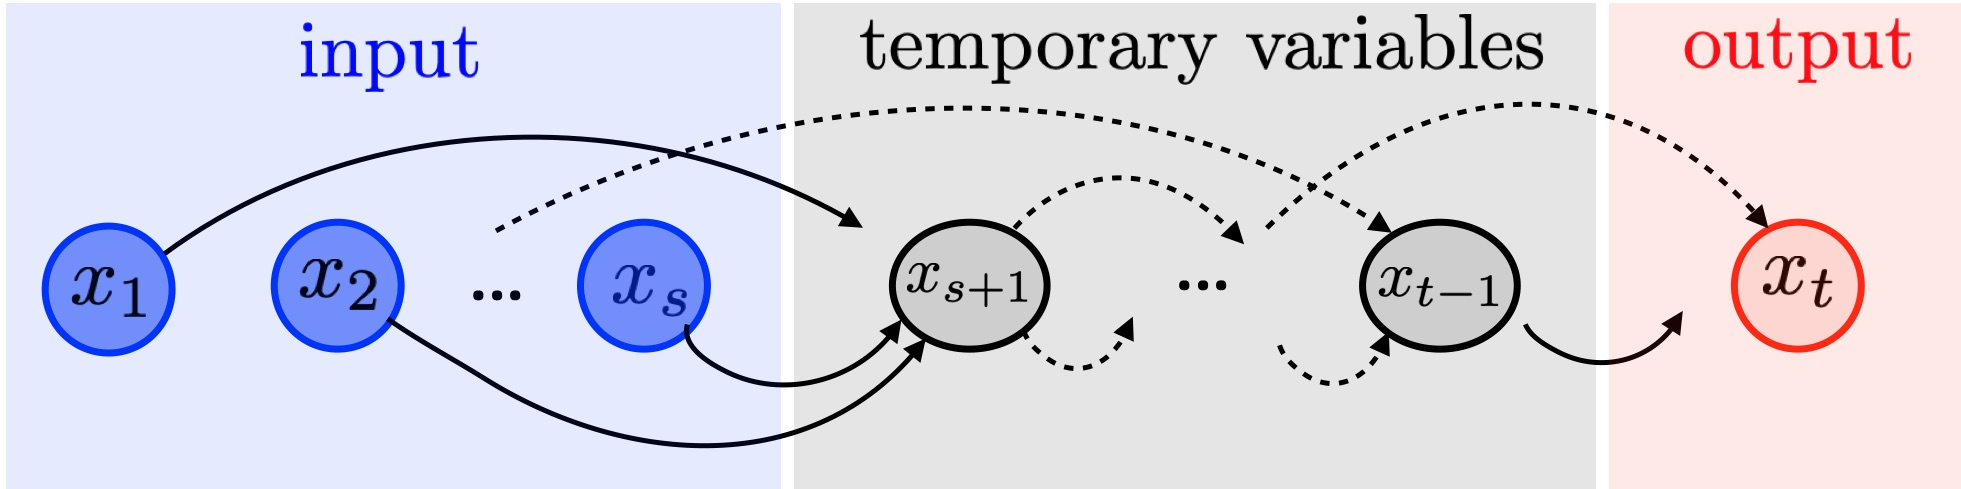
\includegraphics[width=.7\linewidth]{auto-diff/comp-graph}
\caption{\label{fig-compgraph}
A computational graph.
}
\end{figure}

A numerical algorithm can be represented as a succession of functions of the form
\eq{
	\foralls k=s+1,\ldots,t, \quad x_k = f_k( x_1,\ldots,x_{k-1} )
}
where $f_k$ is a function which only depends on the previous variables, see Fig.~\ref{fig-compgraph}. One can represent this algorithm using a directed acyclic graph (DAG), linking the variables involved in $f_k$ to $x_k$. The node of this graph are thus conveniently ordered by their indexing, and the directed edges only link a variable to another one with a strictly larger index.
%
The evaluation of $f(x)$ thus corresponds to a forward traversal of this graph. 
% 
Note that the goal of automatic differentiation is not to define an efficient computational graph, it is up to the user to provide this graph. Computing an efficient graph associated to a mathematical formula is a complicated combinatorial problem, which still has to be solved by the user. Automatic differentiation thus leverage the availability of an efficient graph to provide an efficient algorithm to evaluate derivatives. 



%%%%%%%%%%%%%%%%%%%%%%%%%%%%%%%%%%%%%%%%%%%%%%%%%%%%%%%%%%%%%%%%%%%%%%%%
\subsection{Forward Mode of Automatic Differentiation}

The forward mode correspond to the usual way of computing differentials. It compute the derivative $\pd{x_k}{x_1}$ of all variables $x_k$ with respect to $x_1$. One then needs to repeat this method $p$ times to compute all the derivative with respect to $x_1,x_2,\ldots,x_p$ (we only write thing for the first variable, the method being of course the same with respect to the other ones).

\newcommand{\bk}[1]{\left[#1\right]}
\newcommand{\pdb}[2]{\bk{\pd{#1}{#2}}}

\begin{figure}
\centering
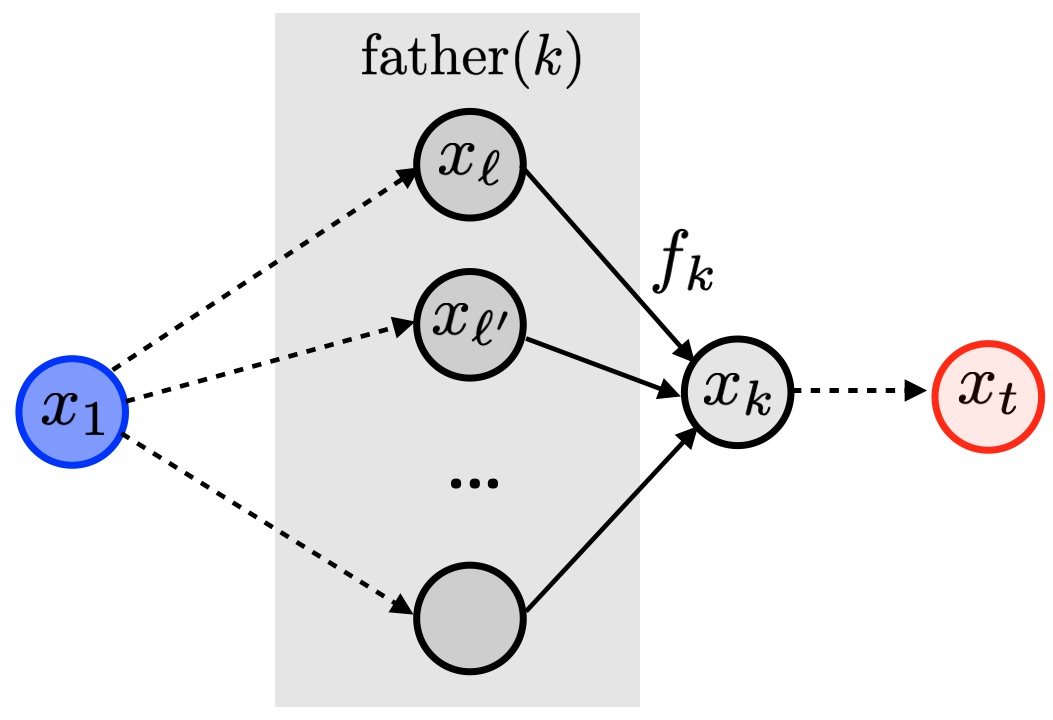
\includegraphics[width=.4\linewidth]{auto-diff/forward-mode}
\quad
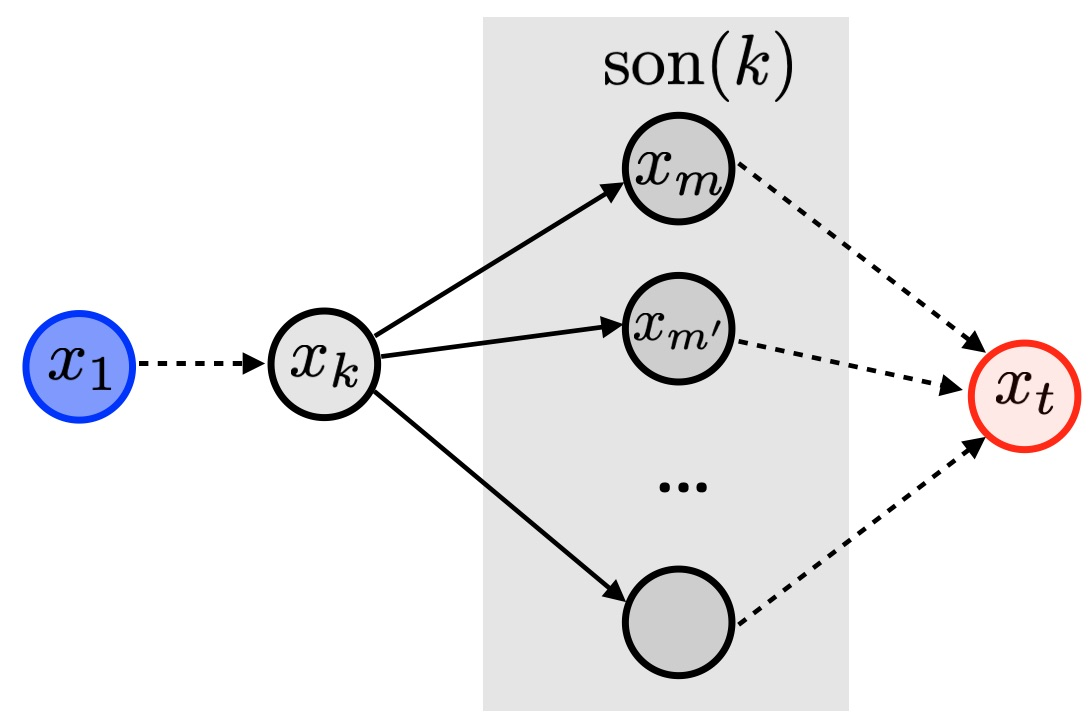
\includegraphics[width=.4\linewidth]{auto-diff/backward-mode}
\caption{\label{fig-forward-backward}
Relation between the variable for the forward (left) and backward (right) modes.
}
\end{figure}

The method initialize the derivative of the input nodes 
\eq{
	\pd{x_1}{x_1} = \Id_{n_1 \times n_1}, \quad 
	\pd{x_2}{x_1} = 0_{n_2 \times n_1}, \ldots, \quad
	\pd{x_s}{x_1} = 0_{n_s \times n_1}, 
}
(and thus 1 and 0's for scalar variables), and then iteratively make use of the following recursion formula
\eq{
	\foralls k=s+1,\ldots,t, \quad
	\pd{x_k}{x_1} 
	= \sum_{\ell \in \text{parent}(k)} \bk{\pd{x_k}{x_\ell}} \times \pd{x_\ell}{x_1}
	= \sum_{\ell \in \text{parent}(k)} \pd{f_k}{x_\ell}(x_1,\ldots,x_{k-1}) \times \pd{x_\ell}{x_1}.
}
The notation ``$\text{parent}(k)$'' denotes the nodes $\ell<k$ of the graph that are connected to $k$, see Figure~\ref{fig-forward-backward}, left. 
%
Here the quantities being computed (i.e. stored in computer variables) are the derivatives $\pd{x_\ell}{x_1}$, and $\times$ denotes in full generality matrix-matrix multiplications.
%
We have put in $[\ldots]$ an informal notation, since here $\pd{x_k}{x_\ell}$ should be interpreted not as a numerical variable but needs to be interpreted as derivative of the function $f_k$, which can be evaluated on the fly (we assume that the derivative of the function involved are accessible in closed form).  

Assuming all the involved functions $\pd{f_k}{x_k}$ have the same complexity (which is likely to be the case if all the $n_k$ are for instance scalar or have the same dimension), and that the number of parent node is bounded, one sees that the complexity of this scheme is $p$ times the complexity of the evaluation of $f$ (since this needs to be repeated $p$ times for $\pd{}{x_1},\ldots,\pd{}{x_p}$). For a large $p$, this is prohibitive. 



%%%
\paragraph{Simple example.}


We consider the fonction 
\eql{\label{eq-simple-func-autodiff}
 	f(x,y) = y\log(x)+\sqrt{y\log(x)}
} 
whose computational graph is displayed on Figure~\ref{fig-dag-example-simple}. The iterations of the forward mode to compute the derivative with respect to $x$ read
\begin{align*}
		\pd{x}{x} &= 1,  \quad \pd{y}{x} = 0 \\
		\pd{a}{x} &= \bk{\pd{a}{x}} \pd{x}{x} = \frac{1}{x} \pd{x}{x} &
			\{x \mapsto a = \log(x)\}\\
		\pd{b}{x} &= \bk{\pd{b}{a}} \pd{a}{x}  + \bk{\pd{b}{y}} \pd{y}{x}  = y \pd{a}{x} + 0 &
			\{(y,a) \mapsto b=ya\}\\
		\pd{c}{x} &= \bk{\pd{c}{b}} \pd{b}{x}  = \frac{1}{2\sqrt{b}} \pd{b}{x}&
			\{b \mapsto c=\sqrt{b}\} \\
		\pd{f}{x} &= \bk{\pd{f}{b}} \pd{b}{x} + \bk{\pd{f}{c}} \pd{c}{x}  = 1\pd{b}{x} + 1\pd{c}{x}&
			\{(b,c) \mapsto f=b+c\}
\end{align*}
One needs to run another forward pass to compute the derivative with respect to $y$
\begin{align*}
		\pd{x}{y} &= 0,  \quad \pd{y}{y} = 1 \\
		\pd{a}{y} &= \bk{\pd{a}{x}} \pd{x}{y} = 0 &
			\{x \mapsto a = \log(x)\}\\
		\pd{b}{y} &= \bk{\pd{b}{a}} \pd{a}{y}  + \bk{\pd{b}{y}} \pd{y}{y}  = 0 + a \pd{y}{y}  &
			\{(y,a) \mapsto b=ya\}\\
		\pd{c}{y} &= \bk{\pd{c}{b}} \pd{b}{y}  = \frac{1}{2\sqrt{b}} \pd{b}{y}&
			\{b \mapsto c=\sqrt{b}\} \\
		\pd{f}{y} &= \bk{\pd{f}{b}} \pd{b}{y} + \bk{\pd{f}{c}} \pd{c}{y}  = 1\pd{b}{y} + 1\pd{c}{y}&
			\{(b,c) \mapsto f=b+c\}
\end{align*}



\begin{figure}
\centering
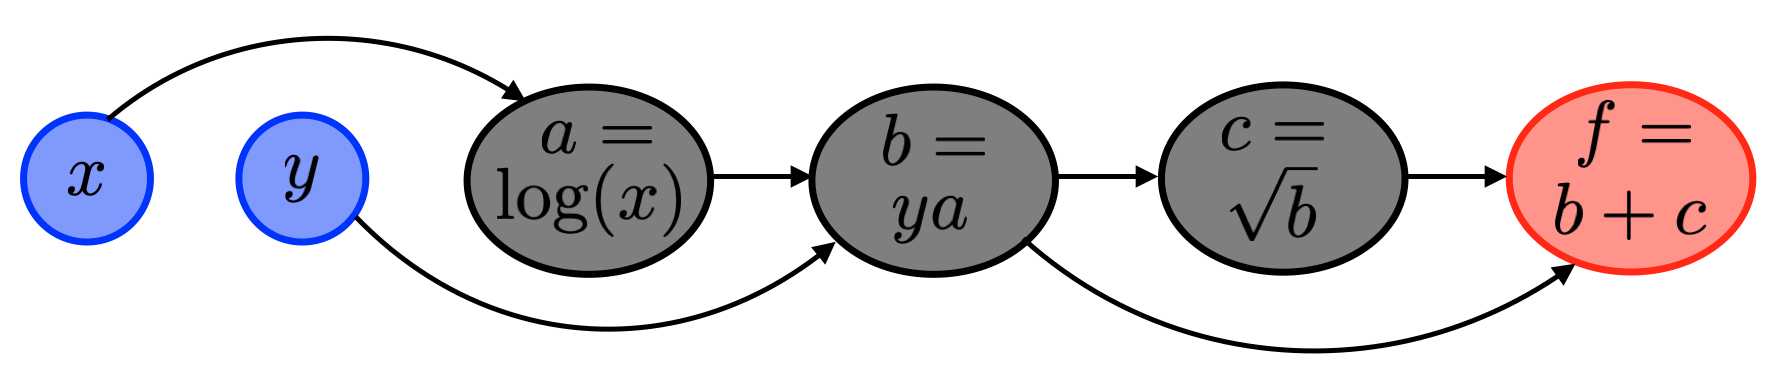
\includegraphics[width=.6\linewidth]{auto-diff/example-simple}
\caption{\label{fig-dag-example-simple}
Example of a simple computational graph.
}
\end{figure}

\if 0
%%%
\paragraph{Simple example.}

We consider the fonction 
\eql{\label{eq-simple-func-autodiff}
 	f(x) = \log(x)+\sqrt{\log(x)}
} 
whose computational graph is displayed on Figure~\ref{fig-dag-example-simple}. The iterations of the forward mode read
\begin{align*}
		\pd{x}{x} &= 1 \\
		\pd{y}{x} &= \bk{\pd{y}{x}} \pd{x}{x} = \frac{1}{x} \pd{x}{x} &
			\{x \mapsto y = \log(x)\}\\
		\pd{z}{x} &= \bk{\pd{z}{y}} \pd{y}{x} = \frac{1}{2\sqrt{y}} \pd{y}{x} &
			\{y \mapsto z=\sqrt{y}\}\\
		\pd{f}{x} &= \bk{\pd{f}{z}} \pd{z}{x} + \bk{\pd{f}{y}} \pd{y}{x} = 1 \pd{z}{x} + 1 \pd{y}{x}&
			\{(x,z) \mapsto f=x+z\}
\end{align*}



\begin{figure}
\centering
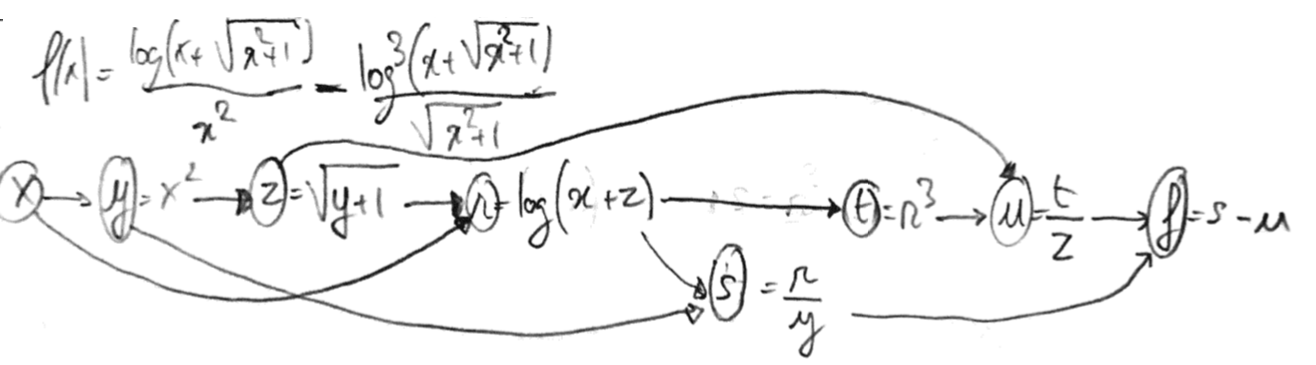
\includegraphics[width=.6\linewidth]{auto-diff/example-complex}
\caption{\label{fig-dag-example-complex}
Example of a more complex computational graph.
}
\end{figure}

%%%
\paragraph{More complex example.}

We now consider the fonction 
\eql{\label{eq-cpx-func-autodiff}
	f(x) = \frac{\log(x+\sqrt{x^2+1})}{x^2} - \frac{\log^3(x+\sqrt{x^2+1})}{\sqrt{x^2+1}}
}
whose computational graph is displayed on Figure~\ref{fig-dag-example-complex}. The iterations of the forward mode read
\begin{align*}
		\pd{x}{x} &= 1 \\
		\pd{y}{x} &= \pdb{y}{x} \pd{x}{x}  = 2 x \pd{x}{x}  &
			\{x \mapsto y = x^2\} \\
		\pd{z}{x} &= \pdb{z}{y} \pd{y}{x} = \frac{1}{2\sqrt{y+1}} \pd{y}{x} &
			\{y \mapsto z=\sqrt{y+1}\}\\
		\pd{r}{x} &= \pdb{r}{z} \pd{x}{x} + \pdb{r}{z} \pd{z}{x} = \frac{1}{x+r} \pd{x}{x} + \frac{1}{x+r} \pd{z}{x}&
			\{(x,z) \mapsto r=\log(x+z)\} \\
		\pd{s}{x} &= \pdb{s}{r} \pd{r}{x} + \pdb{s}{y}\pd{y}{x} = \frac{1}{y} \pd{r}{x} - \frac{r}{y^2}\pd{y}{x} &
			\{ (r,y) \mapsto s=\frac{r}{y}  \} \\
		\pd{t}{x} &= \pdb{t}{r} \pd{r}{x} = 3r^2 \pd{r}{x} &
			\{ r \mapsto t = r^3 \} \\
		\pd{u}{x} &= \pdb{u}{t} \pd{t}{x} + \pdb{u}{z}\pd{z}{x} = \frac{1}{z} \pd{t}{x} - \frac{t}{z^2} \pd{z}{x} &
			\{ (t,z) \mapsto u =  \frac{t}{z}  \} \\
		\pd{f}{x} &= \pdb{f}{s}\pd{s}{x} + \pdb{f}{u}\pd{u}{x} = 1 \pd{s}{x} - 1 \pd{u}{x} &
			\{ (s,u) \mapsto f = s-u \}
\end{align*}
\fi


%%%
\paragraph{Dual numbers.}

A convenient way to implement this forward pass is to make use of so called ``dual number'', which is an algebra over the real  where the number have the form $x + \epsilon x'$ where $\epsilon$ is a symbol obeying the rule that $\epsilon^2=0$. Here $(x,x') \in \RR^2$ and $x'$ is intended to store a derivative with respect to some input variable. These number thus obeys the following arithmetic operations
\eq{
	(x+\epsilon x')(y+\epsilon y') = xy + \epsilon (x y' + y x')
	\qandq
	\frac{1}{x+\epsilon x'} = \frac{1}{x}-\epsilon \frac{x'}{x^2}. 
}
If $f$ is a polynomial or a rational function, from these rules one has that 
\eq{
	f(x+\epsilon) = f(x) + \epsilon f'(x).
}
For a more general basic function $f$, one needs to overload it so that
\eq{
	f(x+\epsilon x') \eqdef f(x) + \epsilon f'(x) x'.
}
Using this definition, one has that 
\eq{
	(f \circ g)(x+\epsilon ) = f(g(x)) + \epsilon f'(g(x))g'(x)
}
which corresponds to the usual chain rule. More generally, if $f(x_1,\ldots,x_s)$ is a function implemented using these overloaded basic functions, one has  
\eq{
	f(x_1+\epsilon,x_2,\ldots,x_s) = f(x_1,\ldots,x_s) + \epsilon \pd{f}{x_1}(x_1,\ldots,x_s)
}
and this evaluation is equivalent to applying the forward mode of automatic differentiation to compute $\pd{f}{x_1}(x_1,\ldots,x_s)$ (and similarly for the other variables).


%%%%%%%%%%%%%%%%%%%%%%%%%%%%%%%%%%%%%%%%%%%%%%%%%%%%%%%%%%%%%%%%%%%%%%%%
\subsection{Reverse Mode of Automatic Differentiation}

Instead of evaluating the differentials $\pd{x_k}{x_1}$ which is problematic for a large $p$, the reverse mode evaluates the differentials  $\pd{x_t}{x_k}$, i.e. it computes the derivative of the output node with respect to the all the inner nodes. 



The method initialize the derivative of the final node
\eq{
	\pd{x_t}{x_t} = \Id_{n_t \times n_t}, 
}
and then iteratively makes use,  from the last node to the first, of the following recursion formula
\eq{
	\foralls k=t-1,t-2,\ldots,1, \quad
	\pd{x_t}{x_k} 
	= \sum_{m \in \text{son}(k)}  \pd{x_t}{x_m} \times \bk{\pd{x_m}{x_k}}
	= \sum_{m \in \text{son}(k)} \pd{x_t}{x_m} \times \pd{f_m(x_1,\ldots,x_m)}{x_k}.
}
%
The notation ``$\text{parent}(k)$'' denotes the nodes $\ell<k$ of the graph that are connected to $k$, see Figure~\ref{fig-forward-backward}, right. 

%%%
\paragraph{Back-propagation.}

In the special case where $x_t \in \RR$, then $\pd{x_t}{x_k} = [\nabla_{x_k} f(x)]^\top \in \RR^{1 \times n_k}$ and one can write the recursion on the gradient vector as follow 
\eq{
	\foralls k=t-1,t-2,\ldots,1, \quad
	\nabla_{x_k} f(x) 
	= \sum_{m \in \text{son}(k)} \pa{\pd{f_m(x_1,\ldots,x_m)}{x_k}}^\top \pa{
	 	\nabla_{x_m} f(x)
	}.
}
where $\pa{\pd{f_m(x_1,\ldots,x_m)}{x_k}}^\top \in \RR^{n_k \times n_m}$ is the adjoint of the Jacobian of $f_m$. This form of recursion using adjoint is often referred to as ``back-propagation'', and is the most frequent setting in applications to ML.

In general, when $n_t=1$, the backward is the optimal way to compute the gradient of a function. Its drawback is that it necessitate the pre-computation of all the intermediate variables $(x_k)_{k=p}^t$, which can be prohibitive in term of memory usage when $t$ is large. There exists check-pointing method to alleviate this issue, but it is out of the scope of this course.

%%%
\paragraph{Simple example.}

We consider once again the fonction $f(x)$ of~\eqref{eq-simple-func-autodiff}, the iterations of the reverse mode read
\begin{align*}
		\pd{f}{f} &= 1 &\\
		\pd{f}{c} &= \pd{f}{f} \pdb{f}{c} = \pd{f}{f} 1 &
			\{ c \mapsto f = b+c\}\\
		\pd{f}{b} &= \pd{f}{c} \pdb{c}{b} + \pd{f}{f} \pdb{f}{b} = \pd{f}{c} \frac{1}{2\sqrt{b}} + \pd{f}{f} 1 & 
			\{ b \mapsto c=\sqrt{b}, b \mapsto f=b+c\} \\
		\pd{f}{a} &= \pd{f}{b} \pdb{b}{a} = \pd{f}{b} y & 
			\{ a \mapsto b=y a\} \\
		\pd{f}{y} &= \pd{f}{b} \pdb{b}{y} = \pd{f}{b} a & 
			\{ y \mapsto b=ya\} \\
		\pd{f}{x} &= \pd{f}{a} \pdb{a}{x} = \pd{f}{a} \frac{1}{x} & 
			\{ x \mapsto a=\log(x)\}
\end{align*}
The advantage of the reverse mode is that a single traversal of the computational graph allows to compute both derivatives with respect to $x,y$, while the forward more necessitates two passes.

\if 0
%%%
\paragraph{More complex example.}

We consider once again the fonction $f(x)$ of~\eqref{eq-cpx-func-autodiff}, the iterations of the reverse mode read
\begin{align*}
		\pd{f}{f} &= 1 &\\
		\pd{f}{u} &= \pd{f}{f} \pdb{f}{u} 
			= \pd{f}{f} (-1) &
			\{u \mapsto f = s-u\}\\
		\pd{f}{t} &= \pd{f}{u} \pdb{u}{t} 
			= \pd{f}{u} \frac{1}{z}  & 
			\{ t \mapsto u= \sqrt{y}, y \frac{t}{z} \} \\
		\pd{f}{s} &= \pd{f}{f} \pdb{f}{s} = \pd{f}{f} 1 & 
			\{ s \mapsto f = s-u \} \\
		\pd{f}{r} &= \pd{f}{t} \pdb{t}{r} + \pd{f}{s} \pdb{s}{r} 
			= \pd{f}{t} 3r^2 + \pd{f}{s} \frac{1}{y} & 
			\{ r \mapsto s = \frac{r}{y}, r \mapsto  t=r^3\}  \\
		\pd{f}{z} &= \pd{f}{u} \pdb{u}{z} + \pd{f}{r} \pdb{r}{z} 
			= \pd{f}{u} \frac{-t}{z^2} + \pd{f}{r} \pdb{1}{x+z} &
			\{ z \mapsto u=\frac{t}{z}, z \mapsto r=\log(x+z)\} \\
		\pd{f}{y} &= \pd{f}{z}\pdb{z}{y} + \pd{f}{s}\pdb{s}{y}
			= \pd{f}{z} \frac{1}{2\sqrt{y+1}} + \pd{f}{s}\frac{-r}{y^2} &
			\{ y \mapsto z=\sqrt{y+1}, y \mapsto s = \frac{r}{y}\} \\
		\pd{f}{x} &= \pd{f}{y}\pdb{y}{x} + \pd{f}{r}\pdb{r}{x}
			= \pd{f}{y} 2x + \pd{f}{r} \frac{1}{x+z}  &
			\{x \mapsto y=x^2, x \mapsto r=\log(x+z)\}		
\end{align*}
\fi


%%%%%%%%%%%%%%%%%%%%%%%%%%%%%%%%%%%%%%%%%%%%%%%%%%%%%%%%%%%%%%%%%%%%%%%%
\subsection{Feed-forward Compositions}

The simplest computational graphs are purely feedforward, and corresponds to the computation of 
\eql{\label{eq-simple-lin-dag}
	f = f_{t} \circ f_{t-1} \circ \ldots \circ f_2 \circ f_1
}
for functions $f_k : \RR^{n_{k-1}} \rightarrow \RR^{n_{k}}$.

The forward function evaluation algorithm initializes $x_0=x \in \RR^{n_0}$ and then computes
\eq{
	\foralls k=1, \ldots, t, \quad x_{k} = f_k(x_{k-1})
}
where at the output, one retrieves $f(x) = x_t$.

Denoting $A_k \eqdef \partial f_k(x_{k-1}) \in \RR^{n_{k} \times n_{k-1}}$ the Jacobian, one has
\eq{
	\partial f(x) = A_{t} \times A_{t-1} \times \ldots A_2 \times A_1.
}
The forward (resp. backward) mode corresponds to the computation of the product of the Jacobian from right to left (resp. left to right) 
\begin{align*}
	\partial f(x) &= A_{t} \times \pa{  A_{t-1} \times \pa{ \ldots \times \pa{ A_3 \times \pa{ A_2 \times A_1 } } } }, \\
	\partial f(x) &= \pa{ \pa{ \pa{ \pa{ A_{t} \times A_{t-1} }  \times A_{t-2} } \times \ldots } \times A_2 } \times A_1.
\end{align*}


\begin{figure}
\centering
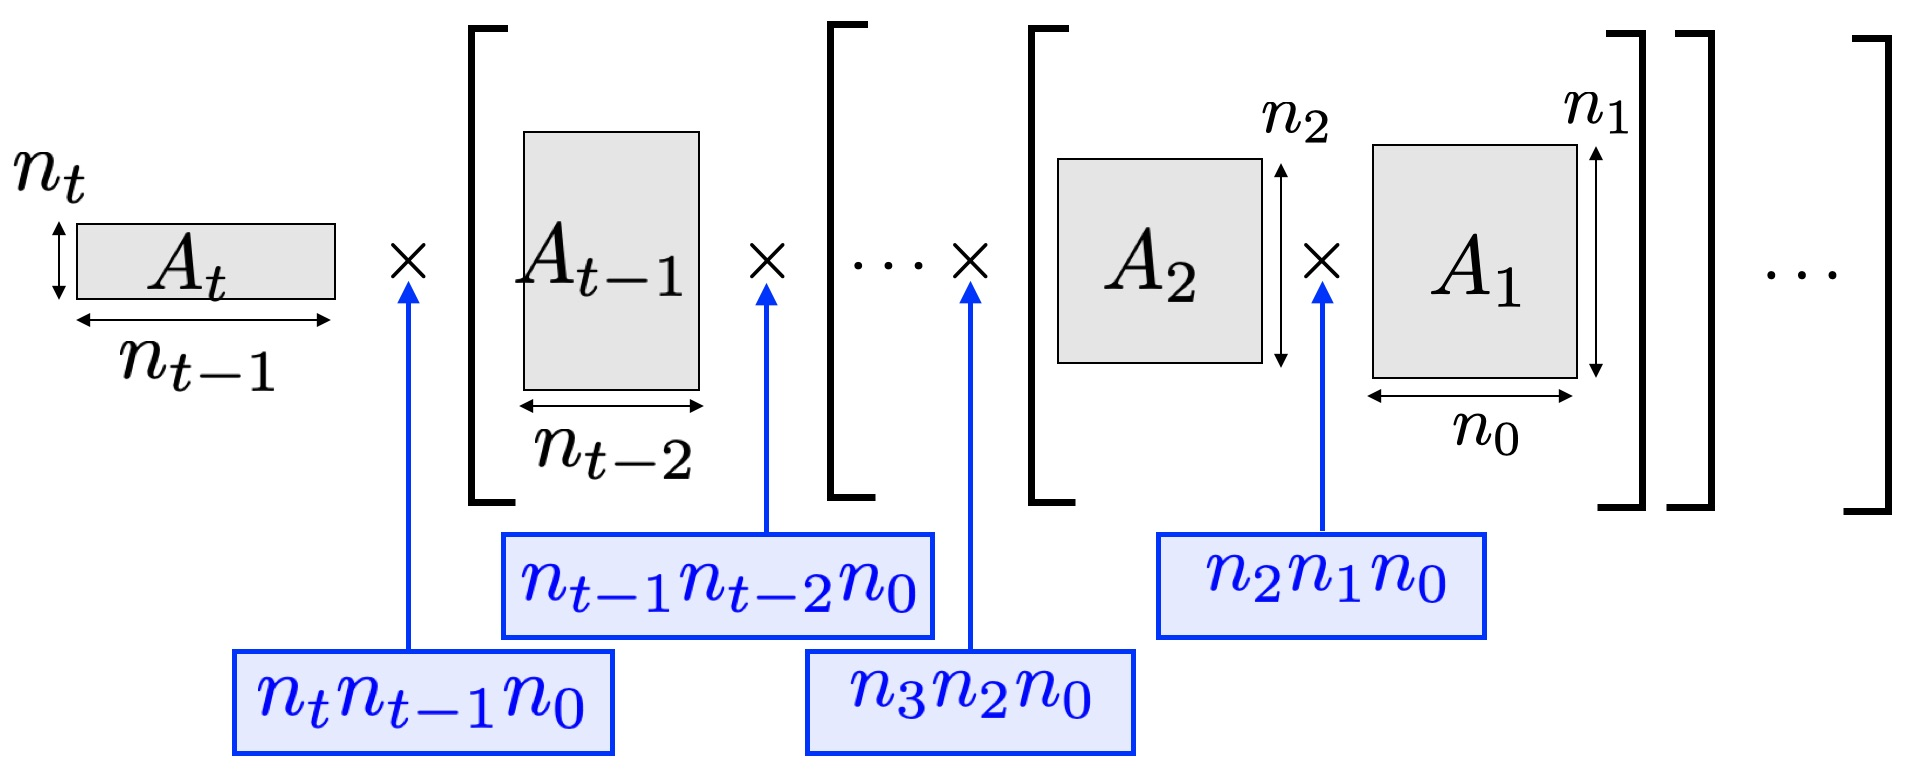
\includegraphics[width=.42\linewidth]{auto-diff/matrix-forward} 
\qquad
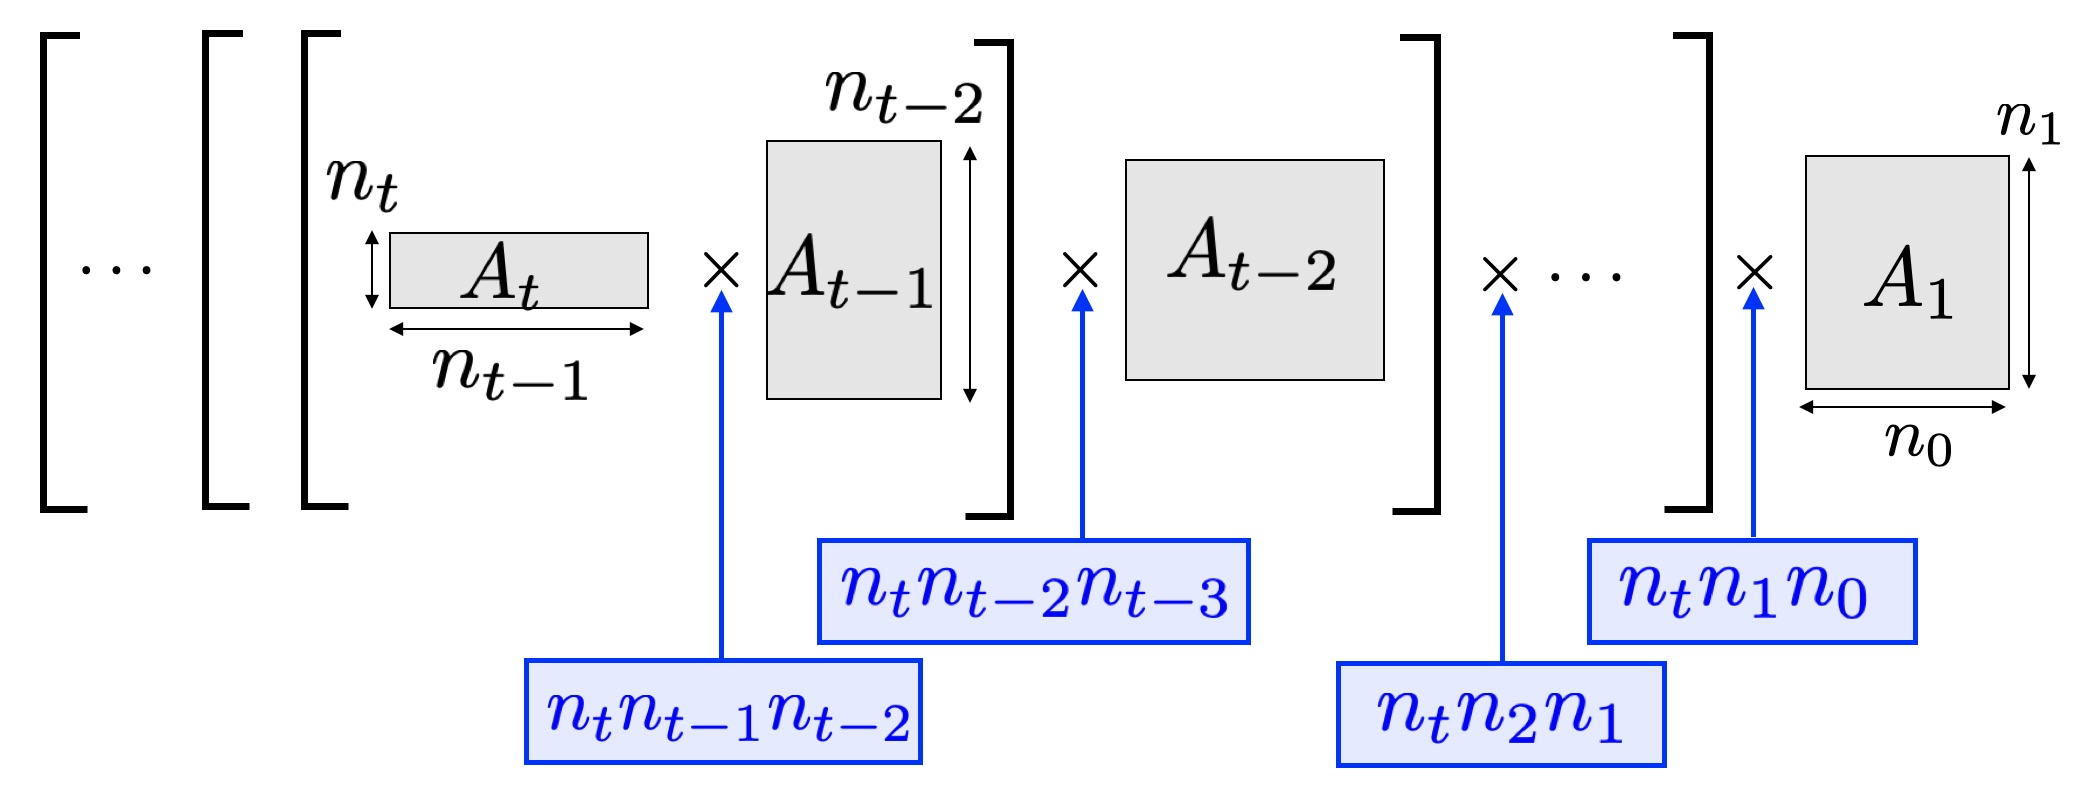
\includegraphics[width=.45\linewidth]{auto-diff/matrix-backward} 
\caption{\label{fig-matrix-mult}
Complexity of forward (left) and backward (right) modes for composition of functions. 
}
\end{figure}

We note that the computation of the product $A \times B$ of $A \in \RR^{n \times p}$ with $B \in \RR^{p \times q}$ necessitates $npq$ operations.
%
As shown on Figure~\ref{fig-matrix-mult}, the complexity of the forward and backward modes are
\eq{
	n_0 \sum_{k=1}^{t-1} n_k n_{k+1}
	\qandq
	n_t \sum_{k=0}^{t-2} n_k n_{k+1}
}
So if $n_t \ll n_0$ (which is the typical case in ML scenario where $n_t=1$) then the backward mode is cheaper. 


%%%%%%%%%%%%%%%%%%%%%%%%%%%%%%%%%%%%%%%%%%%%%%%%%%%%%%%%%%%%%%%%%%%%%%%%
\subsection{Feed-forward Architecture}

We can generalize the previous example to account for feed-forward architectures, such as neural networks, which are of the form
\eql{\label{eq-feednets}
	\foralls k=1, \ldots, t, \quad x_{k} = f_k(x_{k-1},\th_{k-1})
}
where $\th_{k-1}$ is a vector of parameters and $x_0 \in \RR^{n_0}$ is given. The function to minimize has the form
\eql{\label{eq-loss-feedf}
	f(\th) \eqdef L(x_t)
}
where $L : \RR^{n_t} \rightarrow \RR$ is some loss function (for instance a least square or logistic prediction risk) and $\th=(\th_k)_{k=0}^{t-1}$. Figure~\ref{fig-mlp}, top, displays the associated computational graph.


\begin{figure}
\centering
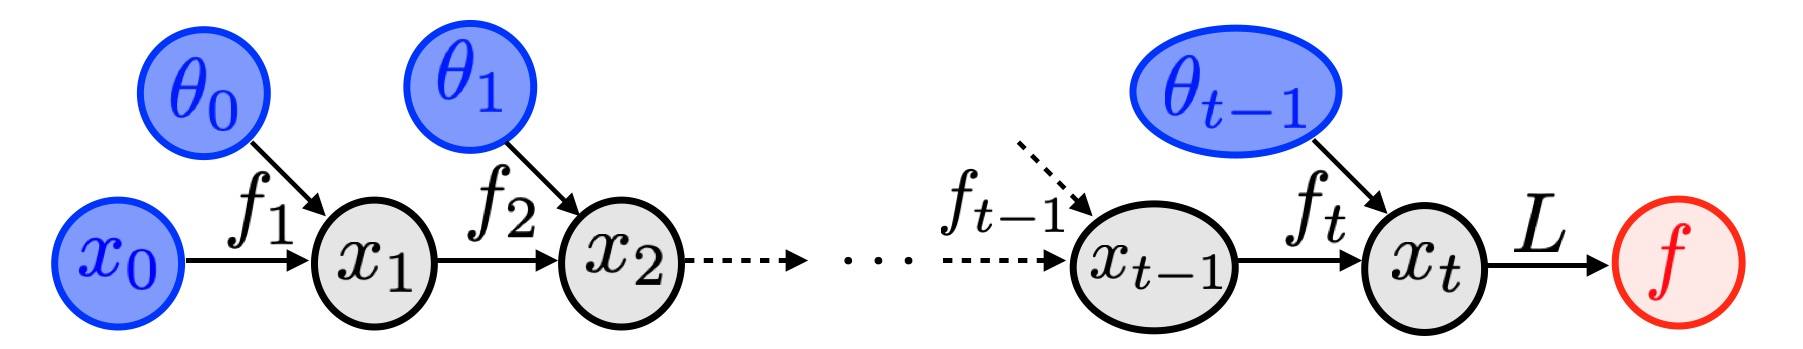
\includegraphics[width=.7\linewidth]{auto-diff/archi-feedforward} 
\caption{\label{fig-mlp}
Computational graph for a feedforward architecture.
}
\end{figure}


One can use the reverse mode automatic differentiation to compute the gradient of $f$ by computing successively the gradient with respect to all $(x_k,\th_k)$. One initializes
\eq{
	\nabla_{x_t} f = \nabla L(x_t) 	
}
and then recurse from $k=t-1$ to $0$
\eql{\label{eq-backprop-discr}
	z_{k-1} = [\partial_x f_k(x_{k-1},\th_{k-1})]^\top z_k
	\qandq
	\nabla_{\th_{k-1}} f = [\partial_\th f_k(x_{k-1},\th_{k-1})]^\top (\nabla_{x_{k}} f)
}
where we denoted $z_k \eqdef \nabla_{x_{k}} f(\th)$ the gradient with respect to $x_{k}$.

%%%
\paragraph{Multilayers perceptron.}

For instance, feedforward deep network (fully connected for simplicity) corresponds to using 
\eql{\label{eq-mlp-func}
	\foralls x_{k-1} \in \RR^{n_{k-1}}, \quad
	f_k(x_{k-1},\th_{k-1}) = \rho( \th_{k-1} x_{k-1} )
} 
where $\th_{k-1} \in \RR^{n_{k} \times n_{k-1}}$ are the neuron's weights and $\rho$ a fixed pointwise linearity, see Figure~\ref{fig-mlp-param}.
%
One has, for a vector $z_k \in \RR^{n_k}$ (typically equal to $\nabla_{x_{k}} f$)
\eq{
	\left\{
	\begin{matrix}
	[\partial_x f_k(x_{k-1},\th_{k-1})]^\top (z_k) = \th_{k-1}^\top w_k z_k, \\
	[\partial_\th f_k(x_{k-1},\th_{k-1})]^\top (z_k) = w_k x_{k-1}^\top
	\end{matrix}
	\right.
	\qwhereq
	w_k \eqdef \diag(\rho'(\th_{k-1} x_{k-1})).
}

\begin{figure}
\centering
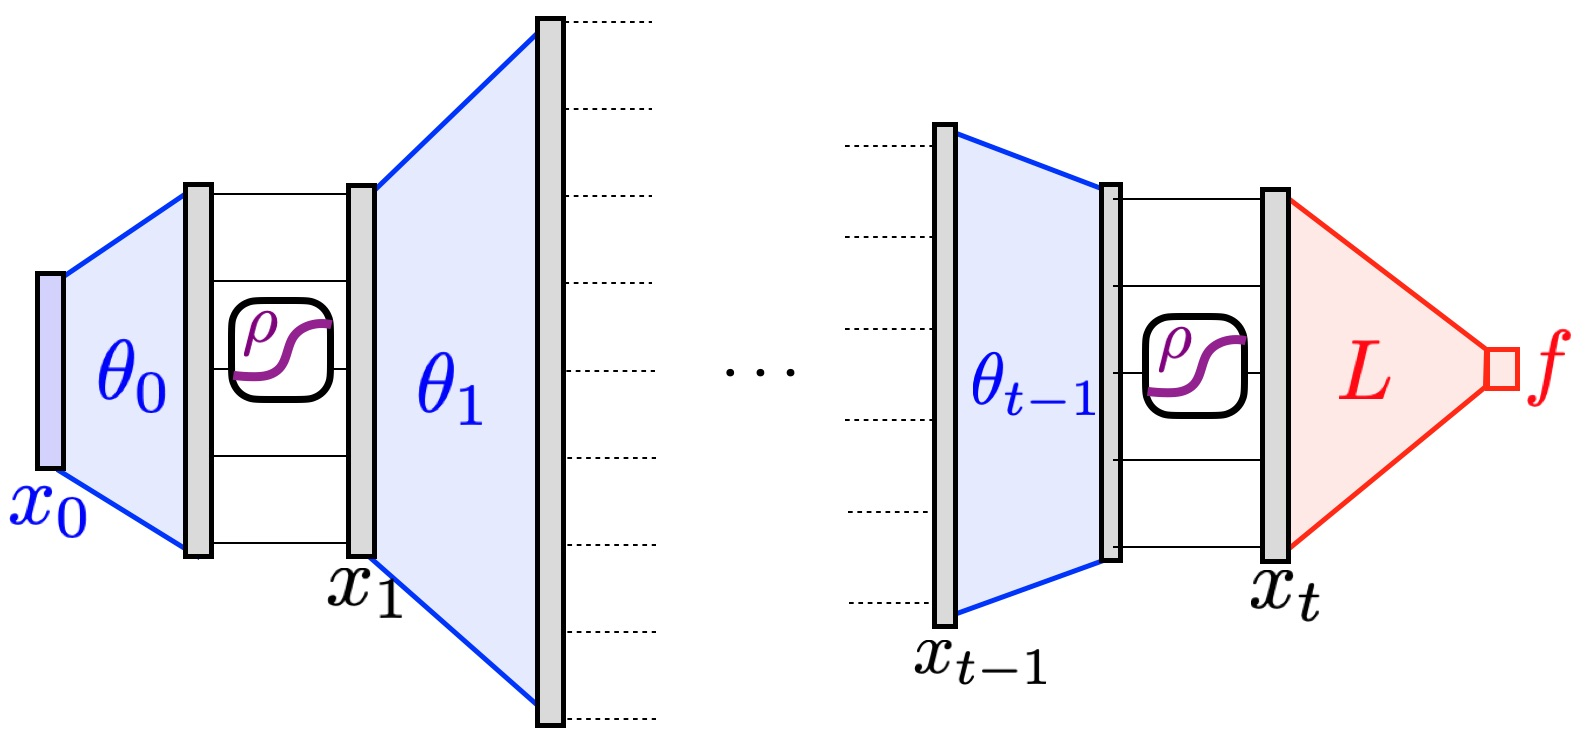
\includegraphics[width=.6\linewidth]{auto-diff/network-mlp} 
\caption{\label{fig-mlp-param}
Multi-layer perceptron parameterization.
}
\end{figure}



%%%
\paragraph{Link with adjoint state method.}

One can interpret~\eqref{eq-feednets} as a time discretization of a continuous ODE. 
%
One imposes that the dimension $n_k=n$ is fixed, and denotes $x(t) \in \RR^n$ a continuous time evolution, so that $x_{k} \rightarrow x(k \tau)$ when $k \rightarrow +\infty$ and $k \tau \rightarrow t$. 
%
Imposing then the structure
\eql{\label{eq-flow-eq}
	f_k(x_{k-1},\th_{k-1}) = x_{k-1} + \tau u(x_{k-1},\th_{k-1}, k\tau)
}
where $u(x,\th,t) \in \RR^n$ is a parameterized vector field, as $\tau \rightarrow 0$, one obtains the non-linear ODE
\eql{\label{eq-ode-structure}
	\dot x(t) = u(x(t),\th(t),t)
}
with $x(t=0)=x_0$.

Denoting $z(t) = \nabla_{x(t)} f(\th)$ the ``adjoint'' vector field, the discrete equations~\eqref{eq-backprop-discr} becomes the so-called adjoint equations, which is a linear ODE 
\eq{
	\dot z(t)  =  - [\partial_x u(x(t),\th(t),t)]^\top z(t)
	\qandq
	\nabla_{\th(t)} f(\th) = [\partial_\th u(x(t),\th(t),t)]^\top z(t).
}
Note that the correct normalization is $\frac{1}{\tau} \nabla_{\th_{k-1}} f  \rightarrow \nabla_{\th(t)} f(\th)$

%%%%%%%%%%%%%%%%%%%%%%%%%%%%%%%%%%%%%%%%%%%%%%%%%%%
\subsection{Recurrent Architectures}

Parametric recurrent functions are obtained by using the same parameter $\th=\th_k$ and $f_k=h$ recursively in~\eqref{eq-mlp-func}, so that 
\eql{\label{eq-feednets-recur}
	\foralls k=1, \ldots, t, \quad x_{k} = h(x_{k-1},\th).
}
We consider a real valued function of the form
\eq{
	f(\th) = L(x_t,\th)
}
so that here the final loss depends on $\th$ (which is thus more general than~\eqref{eq-loss-feedf}).  Figure~\ref{fig-recur}, bottom, displays the associated computational graph.


\begin{figure}
\centering
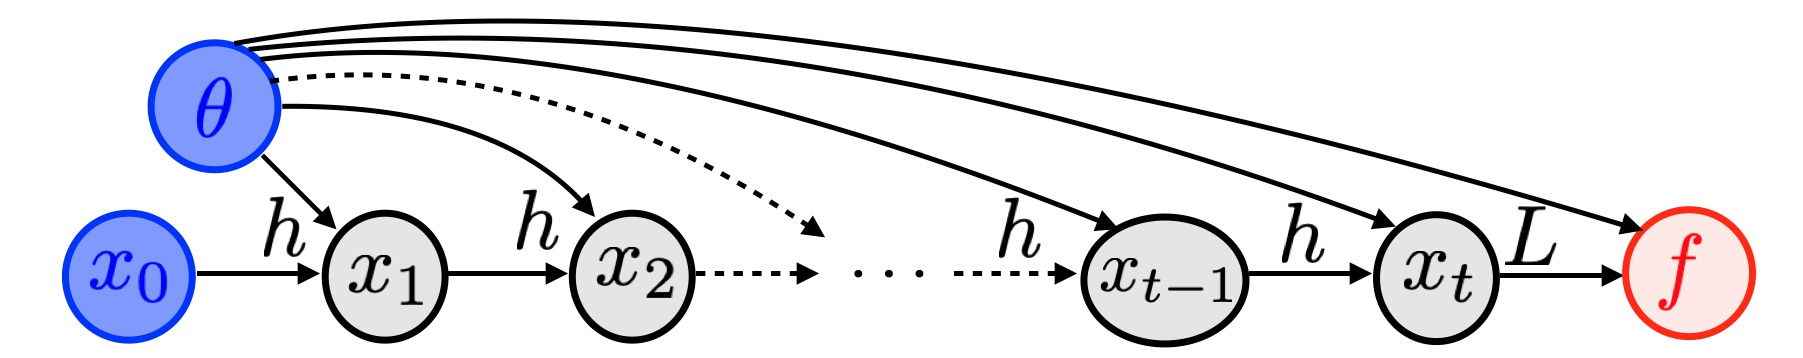
\includegraphics[width=.6\linewidth]{auto-diff/archi-recurrent}
\caption{\label{fig-recur}
Computational graph for a recurrent architecture.
}
\end{figure}

The back-propagation then operates as 
\eql{\label{eq-backprop-discr}
	\nabla_{x_{k-1}} f = [\partial_x h(x_{k-1},\th)]^\top \nabla_{x_{k}} f
	\qandq
	\nabla_{\th} f = 
		\nabla_\th L(x_t,\th) + 
		\sum_k [\partial_\th h(x_{k-1},\th)]^\top \nabla_{x_{k}} f.
}
Similarly, writing $h(x,\th) = x + \tau u(x,\th)$, letting $(k,k\tau) \rightarrow (+\infty,t)$, one obtains the forward non-linear ODE with a time-stationary vector field
\eq{
	\dot x(t) = u(x(t),\th)
}
and the following linear backward adjoint equation, for $f(\th)=L(x(T),\th)$
\eql{\label{eq-jacobian-mlp}
	\dot z(t)  =  - [\partial_x u(x(t),\th)]^\top z(t)
	\qandq
	\nabla_{\th} f(\th) = \nabla_\th L(x(T),\th) + \int_0^T [\partial_\th f(x(t),\th)]^\top z(t) \d t.
}
with $z(0) = \nabla_x L(x_t,\th)$. 

%%%%%
\paragraph{Residual recurrent networks. }

A recurrent network is defined using
\eq{
	h(x,\th) = x + W_2^\top \rho( W_1 x )
}
as displayed on Figure~\ref{fig-recurrent-param}, where $\th = (W_1, W_2) \in (\RR^{n \times q})^2$ are the weights and $\rho$ is a pointwise non-linearity. The number $q$ of hidden neurons can be increased to approximate more complex functions. 
%
In the special case where $W_2=- \tau W_1$, and $\rho=\psi'$, then this is a special case of an argmin layer~\eqref{eq-argmin-layer} to minimize the function $\Ee(x,\th) = \psi( W_1 x )$ using gradient descent, where $\psi(u)=\sum_i \psi(u_i)$ is a separable function.
%
The Jacobians $\partial_\th h$ and $\partial_x h$ are computed similarly to~\eqref{eq-jacobian-mlp}.

\begin{figure}
\centering
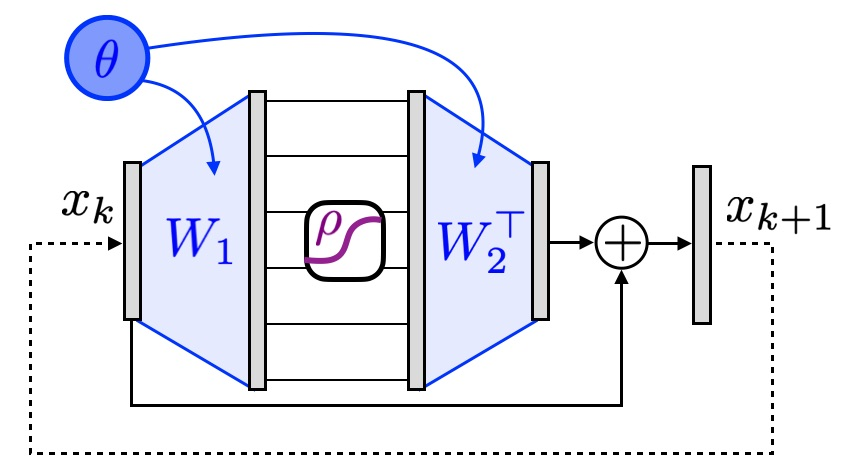
\includegraphics[width=.5\linewidth]{auto-diff/network-recur} 
\caption{\label{fig-recurrent-param}
Recurrent residual perceptron parameterization.
}
\end{figure}


%%%%%
\paragraph{Mitigating memory requirement. }

The main issue of applying this backpropagation method to compute $\nabla f(\th)$ is that it requires a large memory to store all the iterates $(x_k)_{k=0}^t$. A workaround is to use checkpointing, which stores some of these intermediate results and re-run partially the forward algorithm to reconstruct missing values during the backward pass. Clever hierarchical method perform this recursively in order to only require $\log(t)$ stored values and a $\log(t)$ increase on the numerical complexity. 

In some situation, it is possible to avoid the storage of the forward result, if one assume that the algorithm can be run backward. This means that there exists some functions $g_k$ so that 
\eq{
	x_{k} = g_k(x_{k+1},\ldots,x_t).
}
In practice, this function typically also depends on a few extra variables, in particular on the input values $(x_0,\ldots,x_s)$.

An example of this situation is when one can split the (continuous time) variable as $x(t)=(r(t),s(t))$ and the vector field $u$ in the continuous ODE~\eqref{eq-ode-structure} has a symplectic structure of the form $u((r,s),\th,t) = ( F(s,\th,t),G(r,\th,t) )$. One can then use a leapfrog integration scheme, which defines  
\eq{
	r_{k+1} = r_k + \tau F(s_k,\th_k,\tau k)
	\qandq
	s_{k+1} = s_k + \tau G(r_{k+1},\th_{k+1/2},\tau (k+1/2)).
}
One can reverse these equation exactly as
\eq{
	s_k = s_{k+1} - \tau G(r_{k+1},\th_{k+1/2},\tau (k+1/2)).
	\qandq
	r_k = r_{k+1}  - \tau F(s_k,\th_k,\tau k). 
}

%%%%%
\paragraph{Fixed point maps}

In some applications (some of which are detailed bellow), the iterations $x_k$ converges to some $x^\star(\th)$ which is thus a fixed point 
\eq{
	x^\star(\th) = h(x^\star(\th),\th). 
}
Instead of applying the back-propagation to compute the gradient of $f(\th) = L(x_t,\th)$, one can thus apply the implicit function theorem to compute the gradient of $f^\star(\th) = L(x^\star(\th),\th)$. Indeed, one has
\eql{\label{eq-impl-func-formula}
	\nabla f^\star(\th) = [\partial x^\star(\th)]^\top( \nabla_x L(x^\star(\th),\th) )
		 + \nabla_\th L(x^\star(\th),\th).
}
Using the implicit function theorem one can compute the Jacobian as
\eq{
	\partial x^\star(\th) =  - \pa{  \pd{h}{x}(x^\star(\th),\th) }^{-1}  \pd{h}{\th}(x^\star(\th),\th). 
}
In practice, one replace in these formulas $x^\star(\th)$ by $x_t$, which produces an approximation of $\nabla f(\th)$. 
%
The disadvantage of this method is that it requires the resolution of a linear system, but its advantage is that it bypass the memory storage issue of the backpropagation algorithm.



%%%%%
\paragraph{Argmin layers}

One can define a mapping from some parameter $\th$ to a point $x(\th)$ by solving a parametric optimization problem
\eq{
	x(\th) = \uargmin{x} \Ee(x,\th).
}
The simplest approach to solve this problem is to use a gradient descent scheme, $x_0=0$ and
\eql{\label{eq-argmin-layer}
	x_{k+1} = x_k - \tau \nabla \Ee(x_k,\th). 
}
This has the form~\eqref{eq-flow-eq} when using the vector field $u(x,\th) = \nabla \Ee(x_k,\th)$. 

Using formula~\eqref{eq-impl-func-formula} in this case where $h=\nabla \Ee$, one obtains
\eq{
	\nabla f^\star(\th) = -\pa{ \frac{\partial^2 \Ee}{\partial x \partial \th}(x^\star(\th),\th) }^\top 
		\pa{  \pdd{\Ee}{x}(x^\star(\th),\th) }^{-1}
		( \nabla_x L(x^\star(\th),\th) )
		 + \nabla_\th L(x^\star(\th),\th)
}

In the special case where the function $f(\th)$ is the minimized function itself, i.e. $f(\th)=\Ee(x^\star(\th),\th)$, i.e. $L=\Ee$, then one can apply the implicit function theorem formula~\eqref{eq-impl-func-formula}, which is much simpler since in this case $\nabla_x L(x^\star(\th),\th)=0$ so that 
\eql{\label{eq-danskin}
	\nabla f^\star(\th) = \nabla_\th L(x^\star(\th),\th). 
}
This result is often called Danskin theorem or the envelope theorem. 


%%%%%
\paragraph{Sinkhorn's algorithm}

Sinkhorn algorithm approximates the optimal distance between two histograms $a \in \RR^n$ and $b \in \RR^m$ using the following recursion on multipliers, initialized as $x_0 \eqdef (u_0,v_0) = (1_n,1_m)$
\eq{
	u_{k+1} = \frac{a}{K v_k}, \qandq
	v_{k+1} = \frac{b}{K^\top u_k}.
}
where $\frac{\cdot}{\cdot}$ is the pointwise division and $K \in \RR_+^{n \times m}$ is a kernel.
%
Denoting $\th=(a,b) \in \RR^{n+m}$ and $x_k=(u_k,v_k) \in \RR^{n+m}$, the OT distance is then approximately equal to 
\eq{
	f(\th) = \Ee(x_t,\th) \eqdef \dotp{a}{\log(u_t)} + \dotp{b}{\log(v_t)} - \epsilon \dotp{K u_t}{v_t}. 
}
Sinkhorn iteration are alternate minimization to find a minimizer of $\Ee$. 

Denoting  $\Kk \eqdef \begin{pmatrix} 0 & K \\ K^\top & 0 \end{pmatrix} \in \RR^{(n+m) \times (n+m)}$, one can re-write these iterations in the form~\eqref{eq-feednets-recur} using 
\eq{
	h(x,\th) = \frac{\th}{\Kk x}
	\qandq
	L(x_t,\th) = \Ee(x_t,\th)  = \dotp{\th}{\log(x_t)} - \epsilon \dotp{K u_t}{v_t}. 
}
One has the following differential operator 
\eq{
	[\partial_x h(x,\th)]^\top = -\Kk^\top \diag\pa{\frac{\th}{(\Kk x)^2}}, \quad
	[\partial_\th h(x,\th)]^\top = \diag\pa{\frac{1}{\Kk x}}.
}
%\eq{
%	\nabla_x L(x,\th) = ??, \quad
%	\nabla_\th L(x,\th) = ??. 
%}
Similarly as for the argmin layer, at convergence $x_k \rightarrow x^\star(\th)$, one finds a minimizer of $\Ee$, so that $\nabla_x L(x^\star(\th),\th)=0$ and thus the gradient of $f^\star(\th)=\Ee(x^\star(\th),\th)$ can be computed using~\eqref{eq-danskin} i.e.
\eq{
	\nabla f^\star(\th) = \log(x^\star(\th)).
}






% \input{sections/matching}



% \nocite{*}

\bibliographystyle{plain}
\bibliography{all}

\end{document}
